\documentclass[../Report.tex]{subfiles}

\begin{document}


\chapter{Test}
\label{chap:test}


\section{---- firstName ----}
\label{sec:test_firstName}

Diese Zeile teste das paket $ nameref$ mit \nameref{chap:test} und hier mit einer PHANTOMSECTION via \nameref{pha:test.try}---

%\begin{figure}[htb]
%\begin{center}
%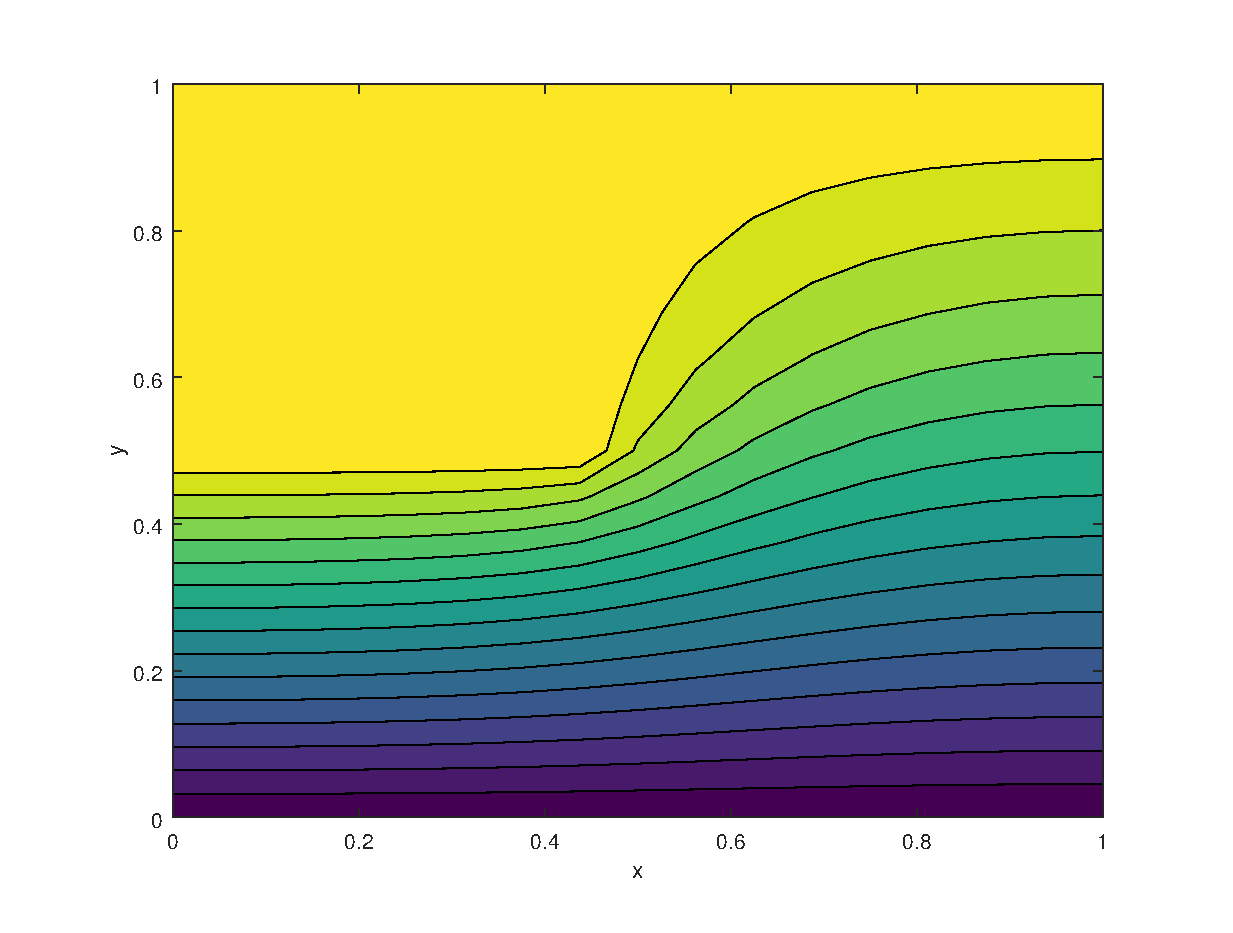
\includegraphics[scale=0.6]{eps/plotPot}
%\end{center}
%\caption[Potentialverlauf eines Kondensators mit Kante]{Potentialverlauf des Kondensators mit Kante.}
%\label{fig:V4.PA4.1}
%\end{figure}
%
%\begin{figure}
%	\centering
%	\begin{tikzpicture}[scale=1]
%		\begin{axis}[
%		xlabel={x},
%		ylabel={mode},
%		%grid=major,
%		cycle multi list={color list\nextlist [1 of]mark list},
%		legend entries={Grundmode},
%		legend style={at={(0.5,-0.2)},anchor=south},
%		]
%		\addplot table[x=x, y=mode1, col sep=comma] {../csv/modes.csv};
%		\addplot+
%%		\addplot+ [
%%mark=ball,
%%mark size=4pt,
%%scatter,% enable scatter
%%scatter src=rand,% the "color data"
%%% configure individual appearances:
%%scatter/use mapped color=
%%{ball color=mapped color}]
%coordinates
%{(-0.1,0) (-1,0.1) (0,0) (0.1,0.1) (0.2,0)};
%
%		
%		
%		\end{axis}
%	\end{tikzpicture}
%	\caption{asdf}
%\end{figure}
%
%
%
%\pgfplotstableread[col sep = comma, columns/3/.style={string type}, ignore chars= {(, ),j}] {transfer_fct.csv}\kennlinie %%%%% cannot deal with a 'j' in imaginary part! %%%
%%\pgfplotstabletypeset[columns={0,3}, columns/3/.style={string type}] \kennlinie
%% erzeugt eine banale Liste
%
%\begin{figure}[hb]
%\centering
%    \begin{tikzpicture}
%\begin{axis}[
%		legend entries = {Amplitude},
%		legend pos = outer north east,
%		extra y tick ={5}
%		extra y tick labels={hier ist $5$}
%		]
%\addplot[blue, thick] table [ x =0, y index=1] {\kennlinie};
%
%		\addplot [red, mark=o, mark size=5pt]coordinates {(10000000, 8)};
%		\addplot coordinates{(20000000, 5)}	;	
%		
%\end{axis}
%\end{tikzpicture}
%\caption{Einzelsinus}
%\end{figure}
%
%Dies ist ein Versuch, eine Transfer-Function zu plotten mittels tikz:

%\begin{figure}[h!]
%\centering
%    \begin{tikzpicture}
%    \datavisualization [scientific axes=clean, 
%    					visualize as line, 
%    					x axis = {attribute = frequency},
%    					y axis = {attribute = amplitude}]
%    	data [read from file = transfer_fct.csv,
%    			%headline = {frequency, amplitude, phaseshift, complex}
%    			];
%    
    
%\begin{axis}[grid=both, xlabel={$t/T_{\textrm{BB}}$},
%ylabel={$\Usin(t)$},                        ytick={-1,1},
%                        yticklabels={$-\widehat{U}$,$\widehat{U}$},
%                        xtick={-4,-2,0,2,4},
%                        xticklabels={-2,-1,0,1,2}]
%\addplot[blue, thick] table [ x expr={\thisrowno{0}}, y
%expr={\thisrowno{1}}, col sep=semicolon] {csv/transfer_fct.csv};
%\end{axis}
%	\end{tikzpicture}
%\caption{Bsp-Plot einer Transfer-Function H}
%  \label{fig:bsp_transfer}
%\end{figure}


Dies ist ein Versuch, ein Frequenzspektrum zu plotten und Marker an relevanten Punkten zu setzen: Hiermit soll die Refernz in Sub-figures versucht werden:
Dies hier soll zu \ref{fig:opt.spektrum_BB_signal} dem Hauptbild referenzieren.\\
Dies hier soll zu \ref{fig:opt.abs_spektrum} dem Betragsspektrum referenzieren.\\
Dies hier soll zu \ref{fig:opt.angle_spektrum} dem Phasen referenzieren.\\


\pgfplotstableread[col sep = comma] {opt_spect_ideal_abs.csv} \absSpectIdeal 
\pgfplotstableread[col sep = comma] {opt_spect_meas_abs.csv} \absSpectMeas
\pgfplotstableread[col sep = comma] {opt_spect_ideal_angle.csv} \angleSpectIdeal 
\pgfplotstableread[col sep = comma] {opt_spect_meas_angle.csv} \angleSpectMeas 
\begin{figure}[htb]
\caption[Spektrum BB-Signal]{Spektrum des Einzelsinus-Signals mit n=109 Punkten}
\label{fig:opt.spektrum_BB_signal}
\begin{subfigure}{0.5 \textwidth}
    \begin{tikzpicture}
\begin{axis}[
		legend entries = {Ideales Signal, Gemessenes Signal},
		legend pos = north east,
		xlabel={Frequenz},
		ylabel={Spektraldichte },
		%xtick distance = 10000000,
		xminorgrids,
		xmajorgrids,
		minor x tick num =3,
		xtick pos = lower,
		ytick pos = left,
		xtick align = outside,
		ytick align = outside,
		scaled x ticks = base 10:-6,
		xtick scale label code/.code={[MHz]},
		xmin = -5000000,
		xmax = 85000000,
%		ymin = 0,
		ymax = 0.03,
		]
		
		\addplot[blue, mark size=3pt] table [ x index =0, y index=1] {\absSpectIdeal};	% plot des Idealen Betragsspektrums
		\addplot[green, mark size=3pt] table [ x index =0, y index=1] {\absSpectMeas};	% Plot des gemessenen Betragsspektrums
\end{axis}
\end{tikzpicture}
\subcaption{Betragsspektren}
	\label{fig:opt.abs_spektrum}
\end{subfigure}
\begin{subfigure}{0.5 \textwidth}
    \begin{tikzpicture}
\begin{axis}[
		legend entries = {Ideales Signal, Gemessenes Signal},
		legend pos = north east,
		xlabel={Frequenz},
		ylabel={Phase},
		%xtick distance = 10000000,
		xminorgrids,
		xmajorgrids,
		minor x tick num =3,
		xtick pos = lower,
		ytick pos = left,
		xtick align = outside,
		ytick align = outside,
		scaled x ticks = base 10:-6,
		xtick scale label code/.code={[MHz]},
		xmin = -5000000,
		xmax = 85000000,
%		ymin = 0,
%		ymax = 0.03,
		]
		
		\addplot[blue, only marks, mark size=1pt] table [ x index =0, y index=1] {\angleSpectIdeal};	% plot des Idealen Betragsspektrums
		\addplot[green, only marks, mark size=3pt] table [ x index =0, y index=1] {\angleSpectMeas};	% Plot des gemessenen Betragsspektrums
\end{axis}
\end{tikzpicture}
\subcaption{Phasenspektrum}
	\label{fig:opt.angle_spektrum}
\end{subfigure}
\end{figure}


\end{document}